\chapter{Projekt}
\label{ch:projekt}

\section{Płytka pomiarowa}

Płytka pomiarowa składa się z dwóch przetworników ADC podłączonych przez odpowiednie interfejsy do wejść komputera Raspberry Pi. Zasilanie układów jest doprowadzone z wyjść zasilających Raspberry Pi. W celu wytłumienia zakłóceń dodano elementy pasywne o odpowiednich wartościach. Sygnały do przetwornika z oscyloskopu doprowadzono przy pomocy kabli BNC i odpowiednich końcówek.
Na Rys. \ref{fig:schplytki} przedstawiono schemat płytki zawierającej przetwornik analogowo-cyfrowy MAX1202 oraz wyjścia cyfrowe i analogowe do podłączenia zewnętrznych czujników. Wyprowadzono także wejścia interfejsu UART w celu komunikacji z komputerem.


\begin{figure}[h]
	\centering
		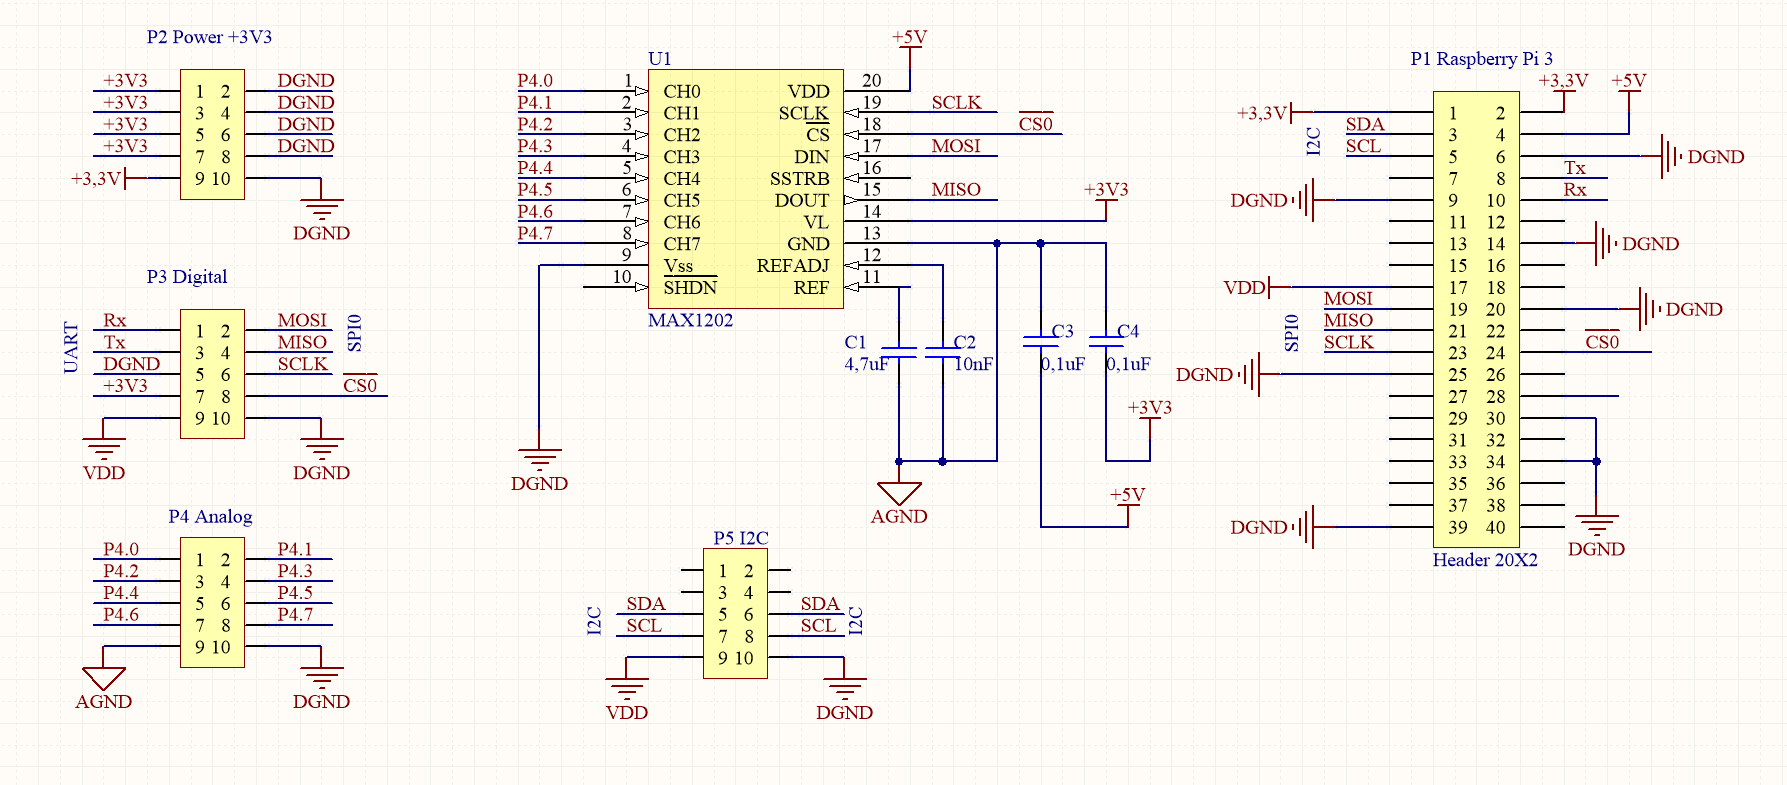
\includegraphics[width=14cm]{schplytki}
	\caption{Schemat płytki dołączanej do Raspberry Pi} 
	\label{fig:schplytki}
\end{figure}

Na Rys.\ref{fig:plytka3d} trójwymiarowy wygląd płytki wygenerowany w programie Altium PCB Designer. 

\begin{figure}[h]
	\centering
		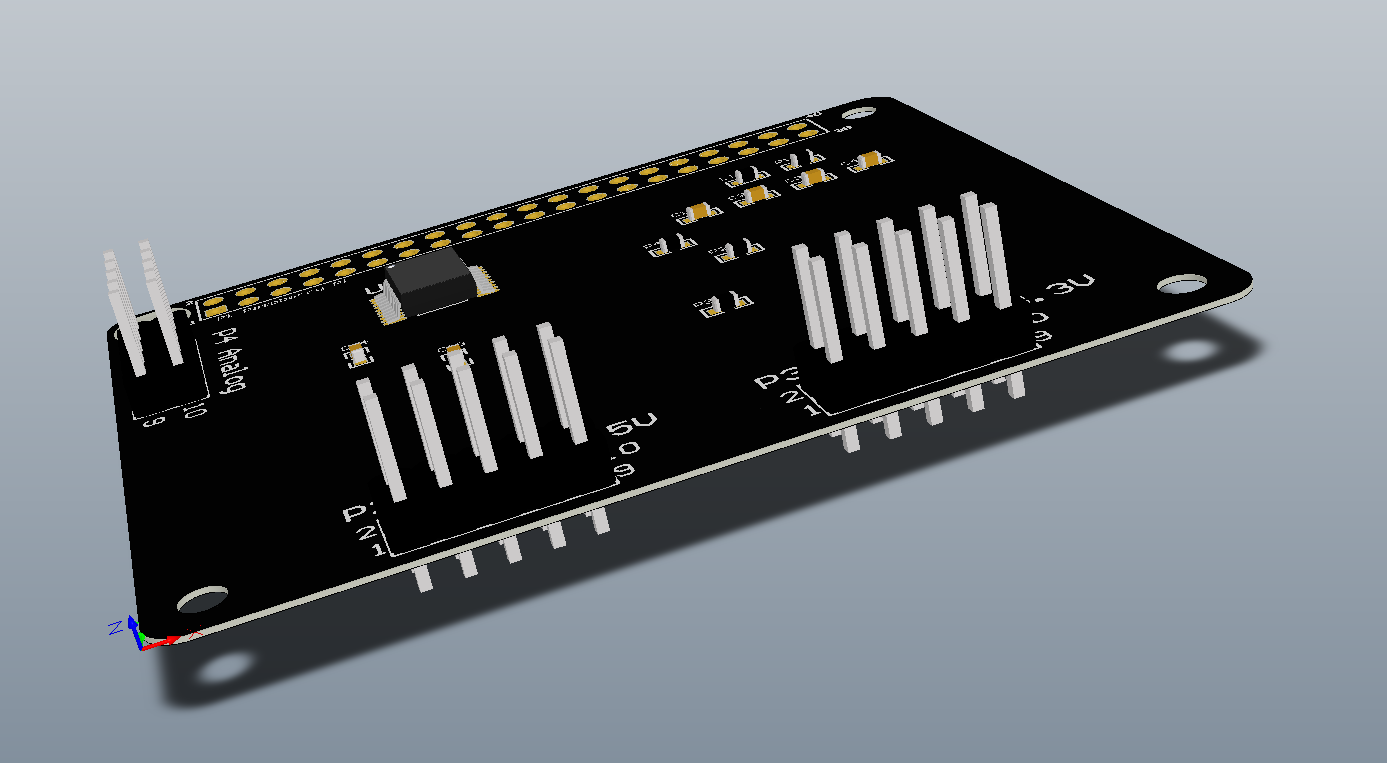
\includegraphics[width=14cm]{plytka3d}
	\caption{Trójwymiarowy wygląd projektu płytki} 
	\label{fig:plytka3d}
\end{figure}

Ze względu na ograniczenia czasowe i optymalizację projektu pod względem kosztu podjęto decyzję zmontowania układu na płytce prototypowej. Wygląd płytki bez zamontowanych elementów przedstawiono na Rys \ref{fig:rpihat}

\begin{figure}[h]
	\centering
		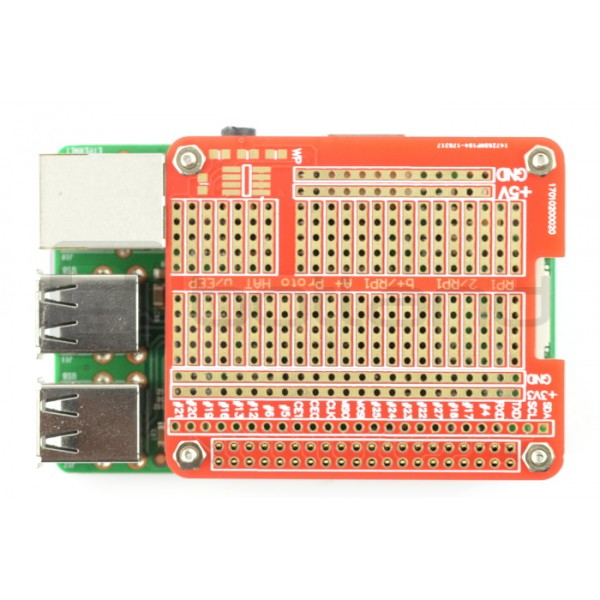
\includegraphics[width=12cm]{rpihat}
	\caption{Płytka prototypowa dołączana do Raspberry Pi 2/3} 
	\label{fig:rpihat}
\end{figure}


\section{Przetwornik analogowo-cyfrowy}

\subsection{Analiza dostępnych układów}
Przy wyborze przetwornika zwrócono uwagę na następujące parametry:
\begin{itemize}
\item cena układu, 
\item rozdzielczość, 
\item częstotliwość próbkowania,
\item interfejs komunikacji,
\item zasilanie i poziomy logiczne
\end{itemize}

\subsection{Przetwornik MAX 1202}

Jednym z wybranych układów był 12-bitowy, 8-kanałowy przetwornik MAX 1202 o próbkowaniu 133 kS/s. Komunikacja z układem odbywa się przez interfejs szeregowy SPI, a poziomy logiczne mogą być ustawione na wartość w zakresie 2,7V - 5,5V w zależności od napięcia podanego na pin VL. Do komunikacji z Raspberry Pi potrzebne są poziomy 3,3V, więc należy podać napięcie 3,3V na odpowiedni pin przetwornika ADC. Układ może być zasilany napięciem 5V.
Podłączenie przetwornika analogowo cyfrowego przez interfejs SPI do platformy Raspberry Pi przebiegało jak na Rys. \ref{fig:maxandrpi} Przetwornik zasilono korzystając z jednego z wyjść +5V dostępnych na płytce. Korzystając z zaleceń producenta zawartych w nocie katalogowej \cite{maxdatasheet} podłączono kondensatory tłumiące niekorzystne dla dokładności pomiaru zakłócenia.  


\begin{figure}[h]
	\centering
		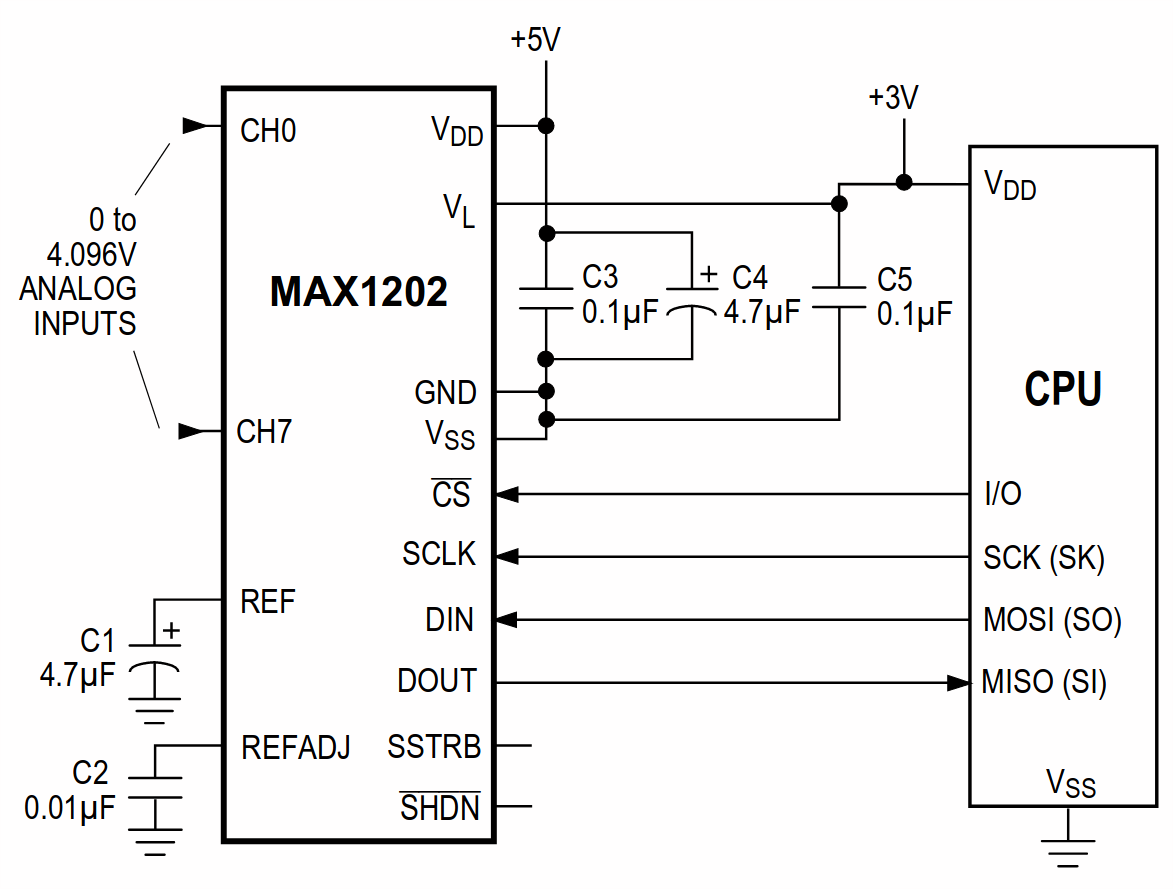
\includegraphics[width=10cm]{max1202_sch}
	\caption{Schemat podłączenia przetwornika MAX1202 do systemu} 
	\label{fig:maxandrpi}
\end{figure}

Na Rys. \ref{fig:maxczasowy} przedstawiono przebiegi czasowe napięć na poszczególnych liniach interfejsu w trakcie jednej konwersji napięcia. Jak widać transmisja jednej próbki napięcia odbywa się za pomocą jednego bajtu konfiguracyjnego wysłanego z układu typu Master. Przetwornik dokonuje konwersji napięcia analogowego z wybranego kanału i wysyła dwa bajty zawierające dane. Z wykresu odczytać można parametr \ang{ACQUISITION} wynoszący 1,5 $\mu$s. 


\begin{figure}[h]
	\centering
		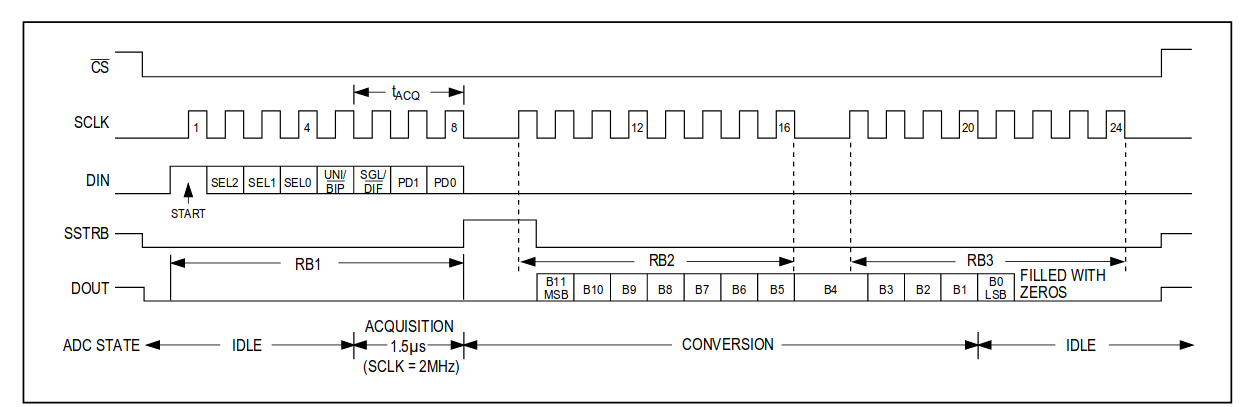
\includegraphics[width=14cm]{max1202time}
	\caption{Wykres czasowy konwersji przetwornika ADC MAX1202} 
	\label{fig:maxczasowy}
\end{figure}


\subsection{Przetwornik MCP 3424}

Drugi testowany układ to 18-bitowy 4-kanałowy przetwornik MCP 3424. Przetwornik komunikuje się z systemem za pomocą interfejsu I2C i posiada wbudowany wzmacniacz programowalny (PGA - z ang Programmable Gain Amplifier). W układzie dostępne jest również źródło napięcia referencyjnego 2.048V oraz oscylator.

\begin{figure}[h]
	\centering
		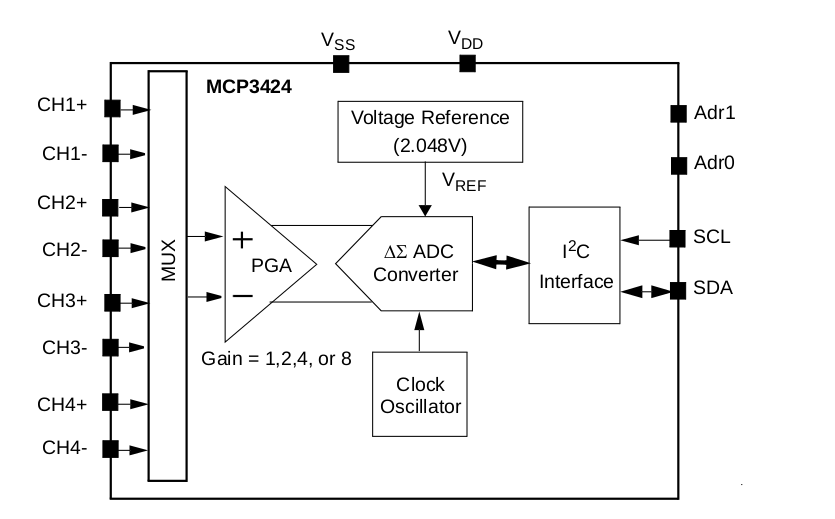
\includegraphics[width=10cm]{mcp3424_fun}
	\caption{Schemat funkcjonalny układu przetwornika MCP3424} 
	\label{fig:uxtouch}
\end{figure}


\begin{table}[t]
\label{tab3.1}
\begin{tabular}{|l|l|l|}

  \hline 
  Nazwa przetwornika & MAX1202 & MCP3424\\
  \hline
  Typ przetwornika & SAR & Sigma Delta\\
  \hline
  Ilość wejść & 8 (4 różnicowe)  & 4 różnicowe \\
  \hline 
  Interfejs komunikacji & SPI & I2C\\
  \hline
  Maksymalna częstotliwość próbkowania & 133 kS/s & 240 SPS (12bit) \\
  \hline
  Wzmacniacz programowalny & brak & x1, x2, x4 lub x8 \\
  \hline
  
\end{tabular}
\caption{Parametry techniczne wybranych przetworników} 
\end{table}


\section{Interfejs SPI}

Interfejs szeregowy SPI (z ang. Serial Peripheral Interface)
jest powszechnie wykorzystywanym synchronicznym interfejsem do komunikacji pomiędzy systemem mikroprocesorowym, a układami peryferyjnymi. Interfejs pozwala na podłączenie tylko jednego układu typu Master komunikującego się z układami typu Slave w trybie full-duplex. Urządzenia podłączone do jednej magistrali muszą mieć jednakowe poziomy logiczne. Transmisja odbywa się za pomocą czterech linii:
\begin{itemize}
\item MOSI (Master In Slave Out), 
\item MOSI (Master Out Slave In),
\item SCLK (Serial Clock),
\item CS (Chip Select).
\end{itemize}


Przetwornik, którego użyto jest w stanie komunikować się przy częstotliwości taktowania zegara do 2MHz.


\section{Interfejs I2C}

Interfejs I2C (również IIC - Inter Integrated Circuit - z ang. pomiędzy układami scalonymi) to synchroniczny interfejs szeregowy zaprojektowany przez firmę Philips. Stosowany jest do komunikacji z urządzeniami nie wymagającymi dużych szybkości transmisji. Interfejs pozwala na podłączenie do magistrali wiele urządzenia typu Master oraz typu Slave. Wszystkie nadajniki posiadają wyjścia typu otwarty kolektor co powoduje, że poziomy logiczne napięć stanu wysokiego układów podłączonych do jednej magistrali mogą się różnić.  Urządzenia komunikujące się za pomocą tego interfejsu mają z góry przypisany adres i są podłączone z resztą urządzeń za pomocą dwóch linii: 
\begin{itemize}
\item SDA (Serial Data Line),
\item SCL (Serial Clock Line).
\end{itemize}


\section{Porównanie dostępnych interfejsów}

Porównanie zostało wykonane pod kątem zastosowania do połączenia układów w systemie akwizycji danych. W tabeli 3.1 przedstawiono zestawienie parametrów technicznych standardów transmisji interfejsów SPI oraz I2C. 


\begin{table}[!ht]
\label{tab3.2}
\begin{tabular}{|l|l|l|}
  \hline 
  Nazwa interfejsu & SPI & I2C\\
  \hline
  Ilość linii sygnałowych & 3 + n(ilość urządzeń)  & 2 \\
  \hline  
  Maksymalna częstotliwość zegara & 125MHz  & 3,2MHz \\
  \hline
  Adresacja urządzeń & linia CS & 10-bitowa  \\
  \hline
  Ilość układów typu Master & 1 & może być wiele\\
  \hline
  Rodzaj transmisji & full-duplex & half-Duplex\\
  \hline
  
\end{tabular}
\caption{Parametry transmisji interfejsów SPI i I2C} 
\end{table}

\section{Pozostałe czujniki podłączane do systemu przez magistralę I2C}

W celu wykonania akwizycji danych pomiarowych wykorzystano dwa moduły z czujnikami ciśnienia, wilgotności powietrza oraz temperatury, podłączonych przez magistralę I2C do komputera Raspberry Pi. Moduły zawierały sensory warunków atmosferycznychw postaci układów scalonych typu MEMS (z ang. Micro Electro-Mechanical System - Mikrosystemy elektromechaniczne).

\subsection{Moduł z czujnikiem ciśnienia i temperatury LPS25H}

Moduł LPS25H od firmy Pololu zawiera barometr mierzący ciśnienie atmosferyczne w zakresie: 260 mbar - 1260 mbar (26 kPa - 126 kPa). W trybie wysokiej rozdzielczości czujnik mierzy z dokładnością 0,2 mbar (0,02kPa). do typową wartością skuteczną szumu 0,01 mbar (1Pa)

\begin{figure}[h]
	\centering
		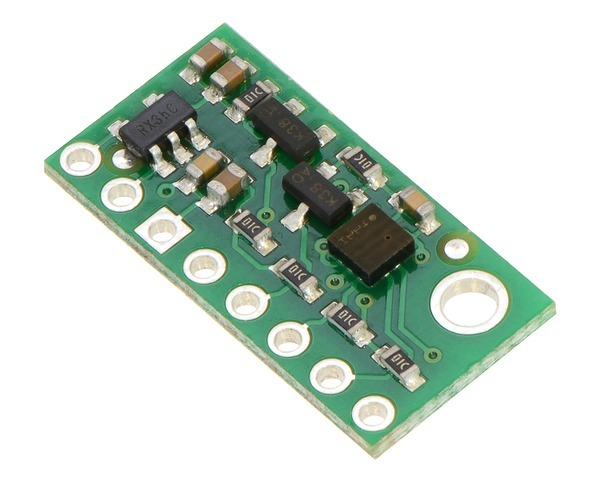
\includegraphics[width=10cm]{pololu}
	\caption{Moduł z czujnikiem ciśnienia i temperatury Pololu LPS25} 
	\label{pic:pololu}
\end{figure}

\subsection{Moduł z czujnikiem wilgotności i temperatury z układem HTS221}

Moduł HTS221 zawiera o sensor wilgotności i temperatury firmy STMicroelectronics, Zakres pomiaru temperatury to 0 - 60\degree C, a wilgotności powietrza: 0 - 100\%. Układ obsługuje interfejsy I2C lub SPI. Na płytce znajduje się konwerter poziomów napięć co umożliwia współpracę układu z urządzeniami o poziomach 3,3V oraz 5V i stabilizator napięcia.

\begin{figure}[t!]
	\centering
		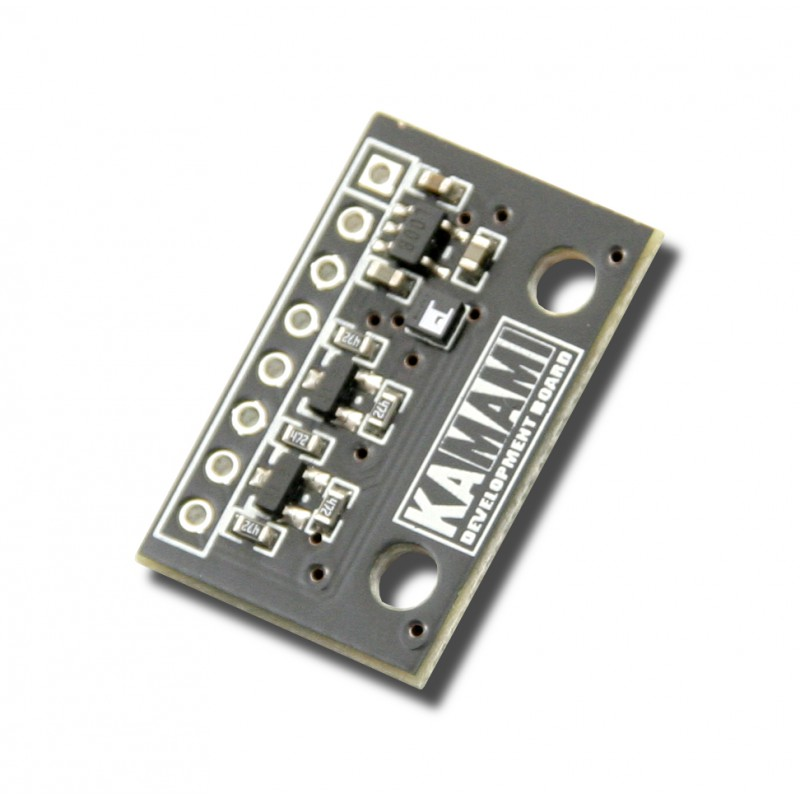
\includegraphics[width=8cm]{hts221}
	\caption{Moduł z czujnikiem wilgotności i temperatury HTS221} 
	\label{pic:hts221}
\end{figure}

Moduły miały podobny rozstaw pinów co umożliwiło podłączenie ich do wspólnej szyny

\begin{figure}[b!]
	\centering
		\includegraphics[width=10cm]{rpiczujniki}
	\caption{Podłączenie zewnętrznych czujników do płytki} 
	\label{pic:rpiczujniki}
\end{figure}
